\chapter{Testes e Resultados}
\label{ch::testes}

%\section{Introdução}
%\label{sec::testes:intro}

Durante a implementação e após a conclusão da versão final do projeto \theapp, foram realizados diversos testes a fim de analisar a exatidão do algoritmo e a qualidade das renderizações obtidas.

Doravante, referir-se-á ao programa final exclusivamente pelo seu nome, \theapp.


\section{Arranque e \textit{Setup} Inicial}
\label{sec::testes::start}

A \theapp~permite modular o seu comportamento através de argumentos passados por linha de comandos. Este é o passo de \textit{setup} inicial do programa.

\begin{itemize}
	\item \verb|-r| (\textit{render mode}): permite definir qual o motor de renderização a ser usado. As opções são:
	\begin{itemize}[nosep]
		\item \verb|CPU|: motor de renderização por \textit{software} (faz usufruto da \ac{CPU});
		\item \verb|GPU|: aceleração por \textit{hardware} (com recurso à \ac{GPU}).
	\end{itemize}
	
	\item \verb|-t| (\textit{threads}): permite definir o número de \textit{threads} a serem usadas no motor de renderização por \textit{software}. Por defeito irá utilizar metade dos núcleos lógicos disponíveis. Caso o utilizador defina um número superior, um aviso é emitido sobre a potencial perda de \textit{performance}.
\end{itemize}

O programa irá carregar todos os recursos necessários ao seu bom funcionamento, em particular:
\begin{itemize}[nosep]
	\item Bibliotecas e \textit{frameworks} (GLFW e \acs{GLAD});
	\item \textit{Shaders} para texto, logótipo e superfície implícita;
	\item Fonte para o texto e imagem do logótipo;
\end{itemize}

Em caso de erro, o programa não arranca e a sua execução é abortada. Em caso de sucesso, é apresentada uma janela com a \textit{home screen} do programa (Figura \ref{fig::home}). O utilizador pode selecionar o ficheiro com as funções a renderizar pressionando a tecla \verb|O|.


\section{Testes em Fase de Desenvolvimento}
\label{sec::teste:dev}

A fase de desenvolvimento englobou duas fases distintas:
\begin{enumerate}[nosep]
	\item Declaração das funções implícitas em código \acs{GLSL} de forma direta no \textit{fragment shader};
	\item Injeção das funções implícitas lidas a partir de ficheiros externos.
\end{enumerate}



\begin{figure}[!htbp]
	\centering
	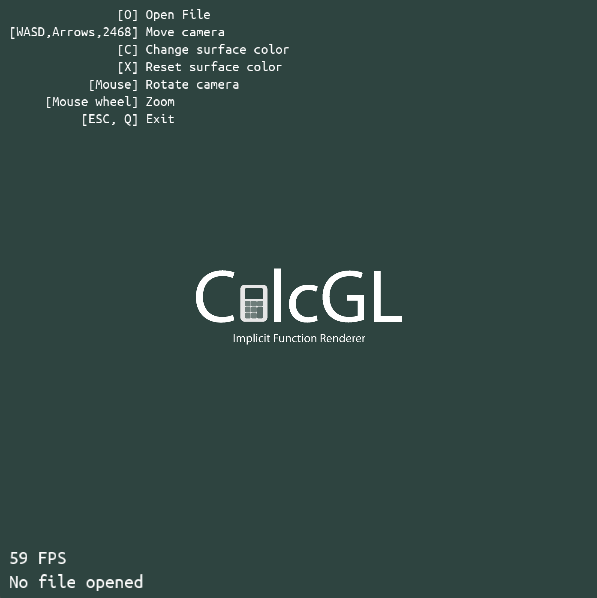
\includegraphics[width=.8\textwidth]{home}
	\caption[Ecrã inicial da aplicação]{Ecrã inicial da aplicação \theapp.}
	\label{fig::home}
\end{figure}

\begin{figure}[!htbp]
	\centering
	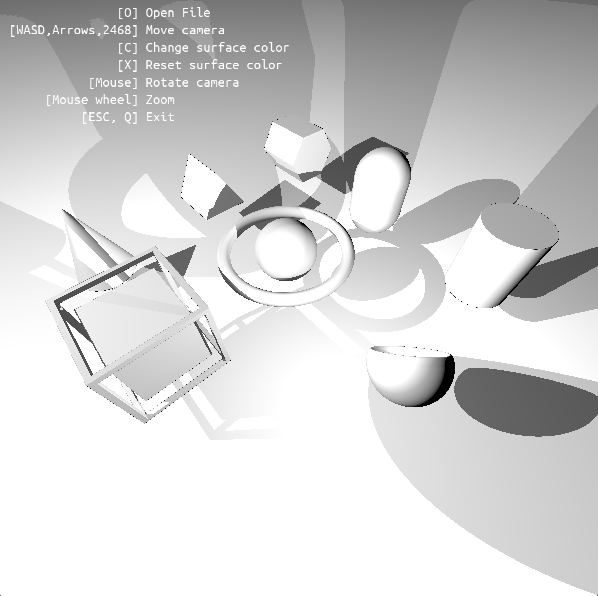
\includegraphics[width=.8\textwidth]{sphereoriginal}
	\caption[Nove objetos com \textit{sphere tracing} no \theapp]{Renderização de nove objetos no \theapp~usando o algoritmo de \textit{sphere tracing}.}
	\label{fig::sphereoriginal}
\end{figure}

\begin{figure}[!htbp]
	\centering
	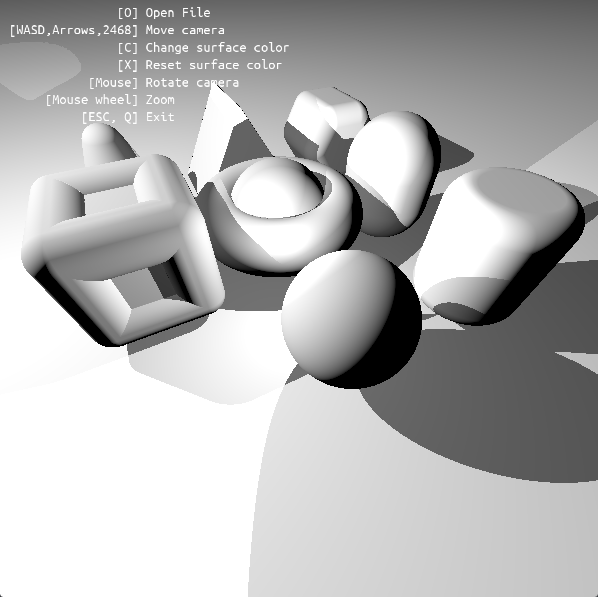
\includegraphics[width=.8\textwidth]{spheresmooth}
	\caption[Nove objetos com \textit{sphere tracing} e suavização no \theapp]{Renderização de nove objetos no \theapp~usando o algoritmo de \textit{sphere tracing} com um fator de suavização $s$ dependente do tempo de execução $t$, em particular $s = \cos(t)$.}
	\label{fig::spheresmooth}
\end{figure}

\begin{figure}[!htbp]
	\centering
	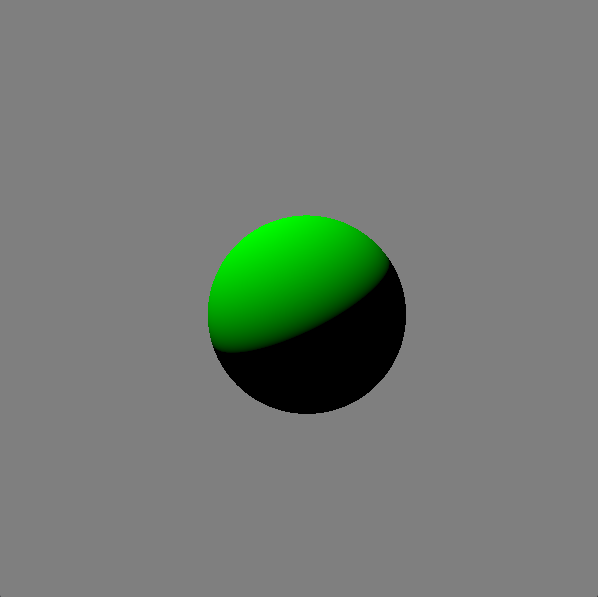
\includegraphics[width=.8\textwidth]{calcglsphere}
	\caption[Esfera no \theapp~com algoritmo naïve]{Esfera renderizada no \theapp, em fase inicial de testes, com o algoritmo naïve.}
	\label{fig::calcglsphere}
\end{figure}

\begin{figure}[!htbp]
	\centering
	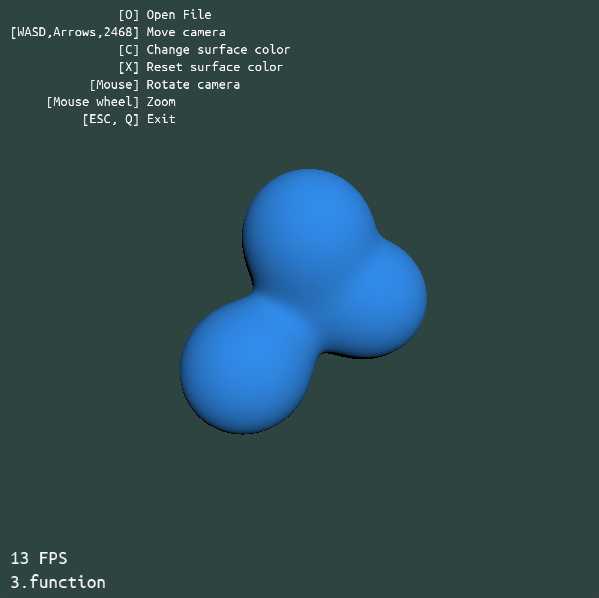
\includegraphics[width=.8\textwidth]{calcglpisurf}
	\caption[Superfície $\Pi$ no \theapp~com algoritmo naïve]{Superfície $\Pi$ renderizada no \theapp~com algoritmo naïve.}
	\label{fig::calcglpisurf}
\end{figure}

\begin{figure}[!htbp]
	\centering
	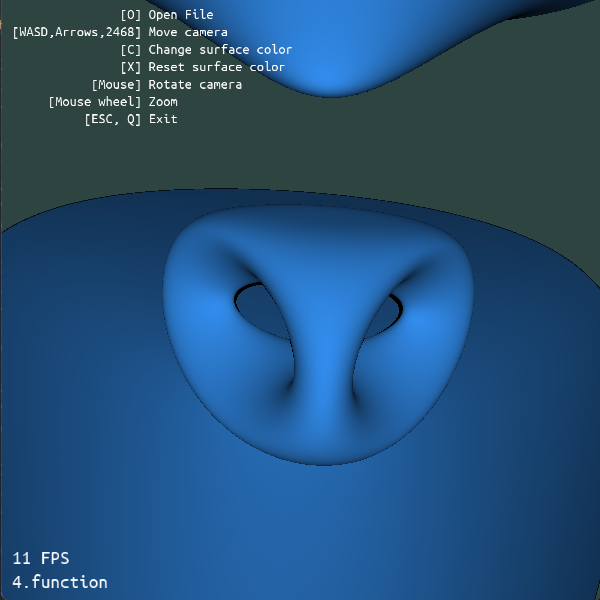
\includegraphics[width=.8\textwidth]{calcglgenus}
	\caption[\textit{Genus} no \theapp~com algoritmo naïve]{\textit{Genus} renderizado no \theapp~com algoritmo naïve.}
	\label{fig::calcglgenus}
\end{figure}




\begin{table}[!htbp]
	\centering
	\caption[Tempos de renderização em \acs{CPU}]{Tempo para a renderização de uma única \textit{frame} com recurso à \acs{CPU} para diferentes números de \textit{threads}. Os testes foram realizados no computador \textit{desktop} listado na Tabela \ref{tab::hardware}.}
	\label{tab::render_cpu}
	\begin{tabular}{r r r}
		\toprule
		\multirow{2}{*}{\textbf{Threads}} & \multicolumn{2}{c}{\textbf{Tempo}} \\
		\cline{2-3}
		& Segundos & h:m's'' \\
		\midrule
		1 &  7087 & 01:58'07'' \\
		2 &  5984 & 01:39'44'' \\
		4 &  7566 & 02:06'06'' \\
		6 & 10414 & 02:53'34'' \\
		\bottomrule
	\end{tabular}
\end{table}


%\section{Conclusões}
%\label{sec::testes:conc}
